\documentclass[pdftex]{article}
\usepackage[T1]{fontenc}
\usepackage[utf8]{inputenc}
\usepackage{graphicx}
\usepackage{caption}

\title{PHYS 721 Homework 2}
\author{Nick Tyler}
\date{}


\begin{document}
\maketitle
\begin{enumerate}
	\item The energy histogram from the first column in data set one was plotted. \\
	\parbox{\linewidth}{\centering
		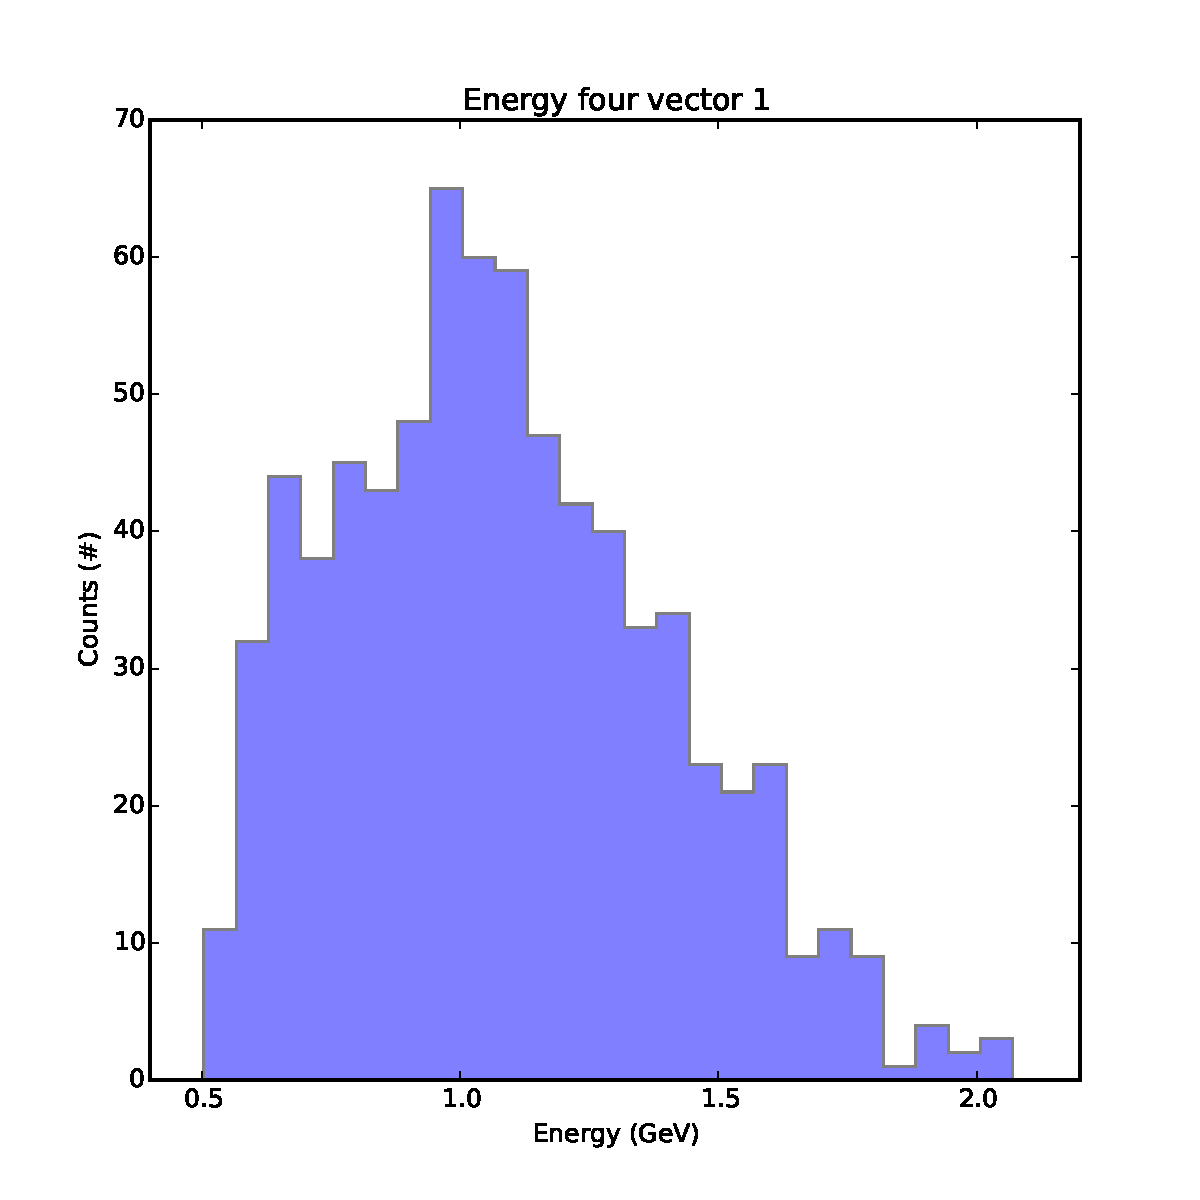
\includegraphics[scale=0.5]{Problem_1.pdf}\\
		\captionof{figure}{Energy Histogram in GeV}
	}
	\newpage
	\item The mass of the four vectors is calculated by finding the magnitude of the four vectors. 
	($m = \sqrt{E^2 - P_x^2 - P_y^2 - P_z^2}$)
	Using ROOT's TLorentzVector class this can easily be done by filling the four vector appropriatly
	and then using the built in magnitude function.  The third histogram represents the mass of the sum of the compenemts
	of the two four vectors.\\
	\parbox{\linewidth}{\centering
		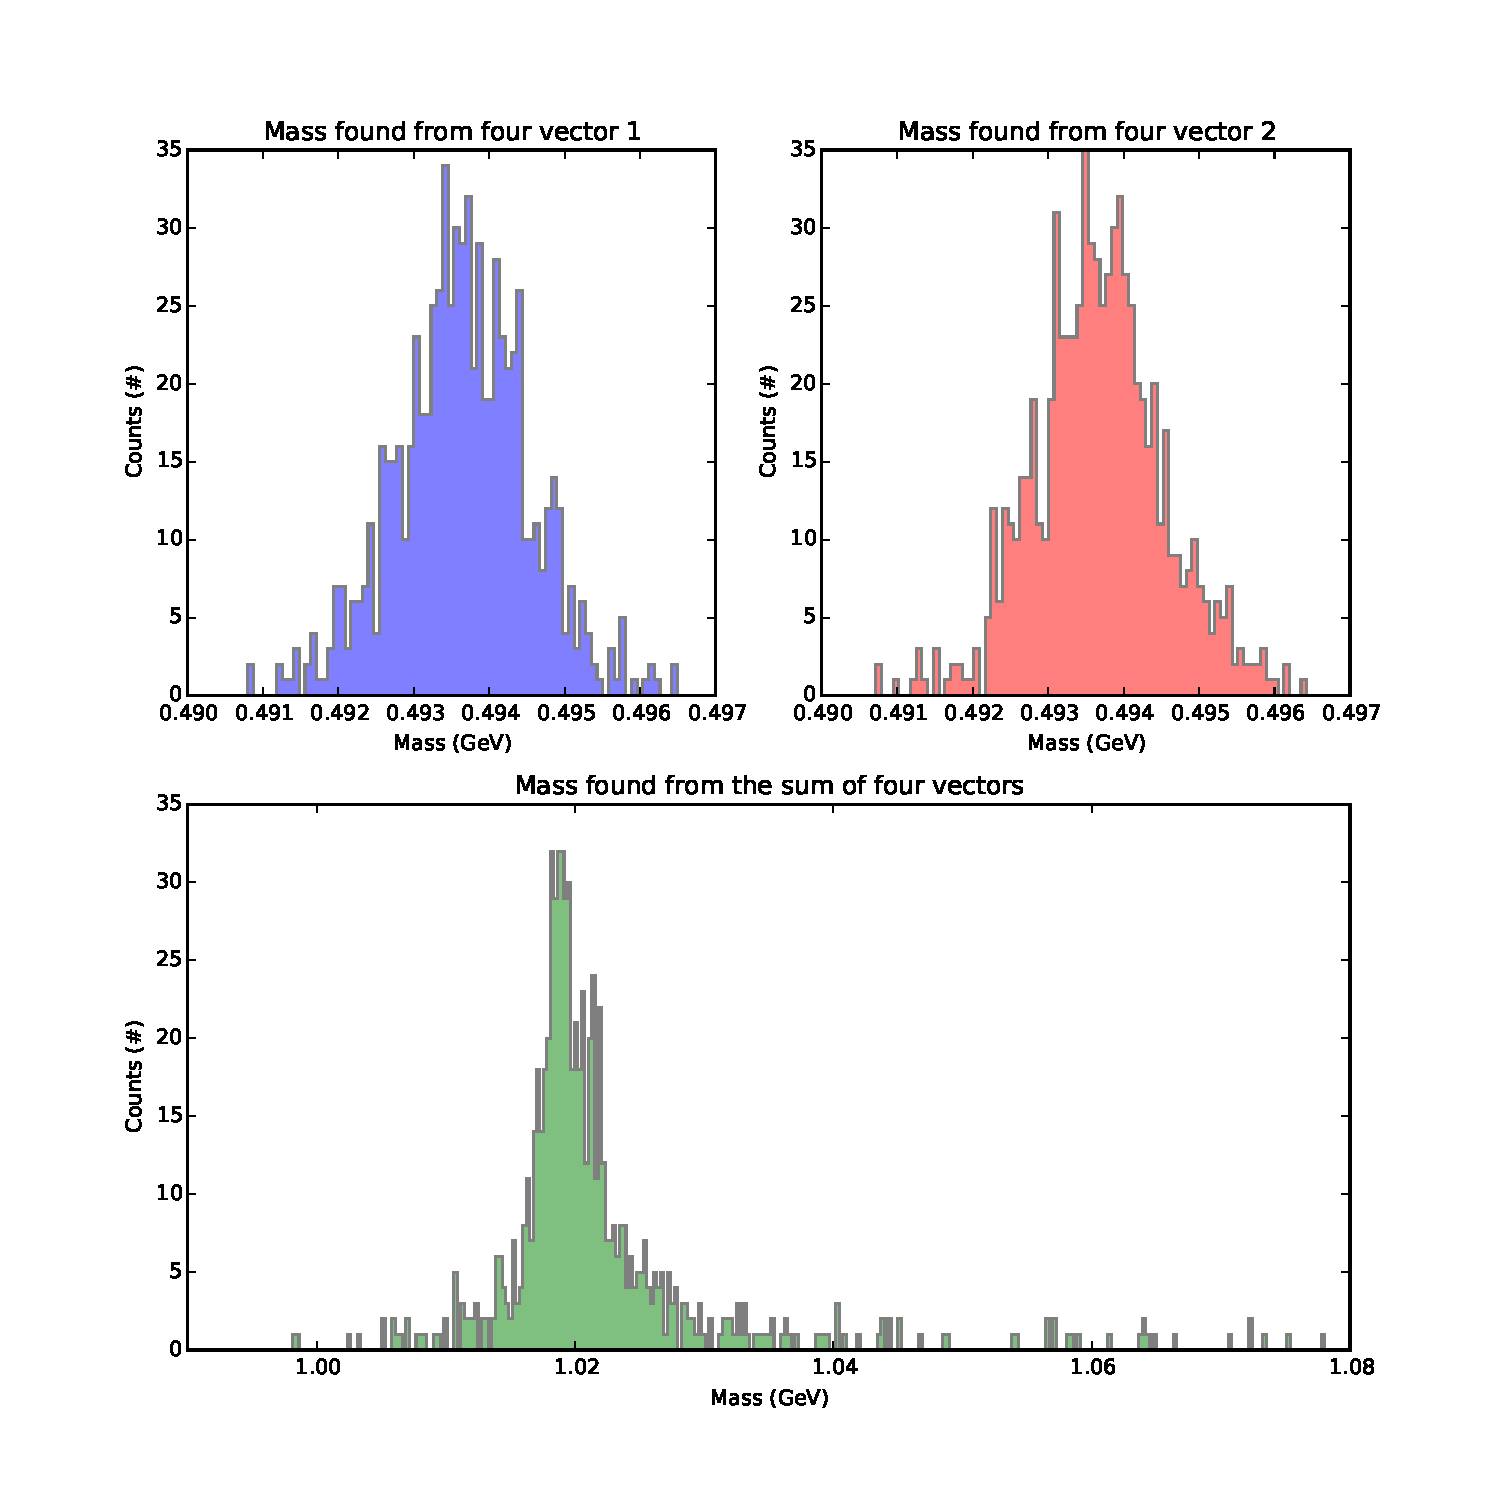
\includegraphics[scale=0.5]{Problem_2.pdf}\\
		\captionof{figure}{Mass Histograms in GeV}
	}

\end{enumerate}

\end{document}